\documentclass[12pt,fleqn]{article}\usepackage{../common}
\begin{document}
Ders 29

Nihayet en son ayristirma (decomposition) konusuna geldik, bu teknik Tekil
Deger Ayristirma (Singular Value Decomposition -SVD-)
teknigidir. Ayristirma su halde olacak

\[ A = U \Sigma V^T \]

Sag tarafta ayrisma sonrasi bir ortogonal matris, bir kosegen (diagonal)
matris, ve tekrar bir ortogonal matris olacak. Yani bildigimiz, sevdigimiz
matris formlari ayrisma sonrasi parcalar olarak elimize gececekler. Ilginc
olan iki tane ortogonal matris elde etmemiz. Ayrica $A$ her turden, her
boyuttan bir matris olabilir (illa karesel olmasi gerekmez mesela).

SVD bu dersin pek cok kavramini da bir araya getirir. Mesela simetrik
pozitif kesin matrisler. Hatirlarsak bu matrisler simetrik oldugu icin
ozvektorleri ortogonal idi. Yani normalde su haldeki bir ayrisma

\[ A = S \Lambda S ^{-1}   \]

Su halde gorulebiliyordu

\[ A = Q \Lambda Q ^{T}   \]

Yani $S$, ortogonal vektorlu $Q$ oluyordu, pozitif kesinlik sayesinde de
normal bir $\Lambda$, icinde sadece pozitif degerler tasiyan bir  $\Lambda$
oluyordu. 

Ozetle, eger $A$ simetrik pozitif kesin ise onun SVD'si $Q \Lambda Q ^{T}$
olacaktir. Bu durumda tek $Q$ matrisi yeterli, diger durumlarda $U,V$ gibi
iki farkli matris lazim. Ayrica sunu da vurgulayalim: SVD icin ortogonallik
aradigimiz onemli bir sart, ``ortogonal carpi kosegen carpi ortogonal''
seklinde bir form istiyorum ozellikle. 

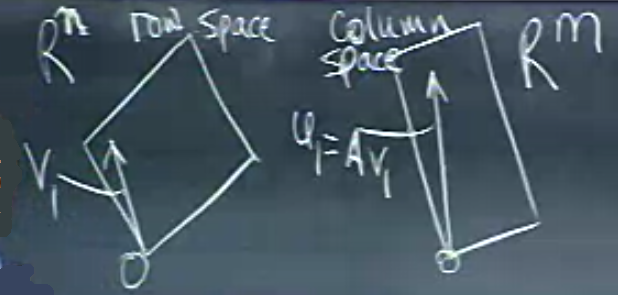
\includegraphics[height=4cm]{29_1.png}

SVD'den bekledigimiz islemi yukaridaki resim uzerinden anlamaya
calisalim. Soldaki duzlem satir uzayi (row space), sagdaki kolon uzayi
(column space). Bir matrisi temsil eden satirlar ve kolonlar bu uzaylarin
icinde. Simdi eger $U \Sigma V^T$ formunu dusunursek, oyle bir kosegen
matris ariyorum ki satir uzayindaki ortogonal bazi (basis) uzayindaki bir
ortogonal baza transform etmeli. Bu hakikaten ozel bir matris olmali.

Soru: satir uzayinin ortogonal bazi var midir? Tabii ki vardir,
Gram-Schmidt tekniginde gorduk, herhangi bir bazin ortogonal bazini
alabiliriz. Ortogonal baz hesabi ozgun degildir, ayni bazdan pek cok
ortogonal baz cikartilabilir, ve satir uzayindaki ``herhangi'' bir
ortogonal bazi alip kolon uzayina transform edersem onun illa ortogonal
kalacagi garanti degildir. Yani transform edildikten sonra da ortogonal
kalacak ozel bir ortogonal baz ariyorum. Yapmaya calistigim carpim her
vektoru gosterecek sekilde nasildir?

\[ 
A \left[\begin{array}{rrrr}
&&& \\
v_1 & v_2& ... & v_r \\
&&& 
\end{array}\right] = 
\left[\begin{array}{rrrr}
&&& \\
u_1 & u_2& ... & u_r \\
&&& 
\end{array}\right] 
\left[\begin{array}{rrrr}
\sigma_1 &&& \\
 & \sigma_2&  & \\
&& \ddots & \\
&&& \sigma_r
\end{array}\right] 
 \]

Yani $Av_1$ carpimi bana $u_1 \sigma_1$'i vermeli. Matris olarak yukaridaki 

\[ AV = U\Sigma \]

Hatta ortogonallikten daha ileride ortonormalligi hesaplamak daha da iyi. 

Ornek 

\[ 
A = 
\left[\begin{array}{rr}
4 & 4 \\ -3 & 3
\end{array}\right]
 \]

$A$ tersine cevirilebilir (invertible) o zaman kertesi (rank)
2. Aradiklarim 

\[ v_1,v_2 \  \mathbb{R}^2 \textit{ satir uzayinda }  \]

\[ u_1,u_2 \  \mathbb{R}^2 \textit{ kolon uzayinda }  \]

\[ \sigma_1 > 0, \sigma_2 > 0 \]

Sifir uzayi (nullspace) burada problem degil. Zorluklar neler? Matris
simetrik olmayabilir, o zaman ozvektorleri kullanamam, cunku onlar
ortogonal degildir.

\[ A = U \Sigma V^{-1} \]

$V^{-1}$'yi baska nasil yazabilirim? $V$ kare, ortogonal olacagina gore,
$V^{-1} = V^{T}$. O zaman 

\[ A = U \Sigma V^{T} \]

Simdi hesabi dusunmeye baslayalim. Iki tane ayri ortogonal matris bulmam
lazim, ama bunlarin ikisini de ayni anda bulmak istemiyorum. Bir fikir:
oyle bir numara yapayim ki $U$ yokolsun her sey $V$ uzerinden temsil
edilsin. 

Alttaki ifade ne zaman elimizde genel dikdortgensel (kare olmayan) bir
matris varsa karsimiza cikan bir ifade, $A^TA$. Bu matris kare, pozitif
kesin, yani guzel ozellikleri var. O zaman ustteki formulu $A^T$ ile soldan
carpacagiz,

\[ A^T = V \Sigma^T U^{T}  \]

olduguna gore,

\[ A^TA = V \Sigma^T U^{T}  U \Sigma V^{T}  \]

$U^TU = I$ olduguna gore

\[ A^TA = V \Sigma^T \Sigma V^{T}  \]

Kolaylastirmalar bitmedi. $\Sigma$ kosegen olduguna gore, $\Sigma^T\Sigma$
kosegendeki degerlerin karesinden ibarettir. 

\[ = V 
\left[\begin{array}{rrrr}
\sigma_1^2 &&& \\
 & \sigma_2^2 &  & \\
&& \ddots & \\
&&& \sigma_r^2 
\end{array}\right] 
V^T
  \]

Iste, $U$'lar yokoldu. Bu son ulastigimiz formda $V$'ler nedir?
Ozvektorlerdir! Problem mukemmel bir ozdeger / ozvektor problemine
donustu, yani $Q\Lambda Q$ haline geldi. Bu kolayliga, sonuca $A$ yerine $A^TA$'yi
kullanmak sayesinde eristik.

Pekala bu sekilde $V$'leri elde ediyoruz, ama $U$'yu nasil elde edecegiz?
Onu gecici bir sure icin yokettik, ama $U$ hala hesaplamamiz gereken bir
buyukluk, vektorler. Onun da caresi var, $A^T$ ile soldan carpmak yerine ana
formulu $A^T$ ile sagdan carparsak, bu sefer $V$'ler yokolur, ve yine
benzer ozdeger / ozvektor hesabina geliriz, ama bu sefer $U$ hesaplariz.

\[ AA^T = U\Sigma V^TV\Sigma^TU^T \]

\[  = U\Sigma \Sigma^TU^T \]

Ornek icin tum bu hesaplari yapalim. 

\[ A^TA = 
\left[\begin{array}{rr}
4 & -3 \\ 4 & 3
\end{array}\right]
\left[\begin{array}{rr}
4 & 4 \\ -3 & 3
\end{array}\right] = 
\left[\begin{array}{cc}
25 & 7 \\ 7 & 25
\end{array}\right]
 \]

Ozvektorler

\[ 
\left[\begin{array}{r}
1 \\ 1
\end{array}\right],
\left[\begin{array}{r}
-1 \\ 1
\end{array}\right]
 \]

Ozdegerler

$\lambda_1=32, \lambda_2=18$. 

Ozvektorleri normalize etmeli

\[ 
\left[\begin{array}{r}
1 / \sqrt{ 2} \\ 1/ \sqrt{ 2}
\end{array}\right],
\left[\begin{array}{r}
-1/ \sqrt{ 2} \\ 1/ \sqrt{ 2}
\end{array}\right]
 \]

o zaman 

\[ 
\underbrace{
\left[\begin{array}{rr}
4 & 4 \\ -3 & 3
\end{array}\right] 
}_{A}
=
\underbrace{
\left[\begin{array}{rr}
 &  \\  & 
\end{array}\right]
}_{U}
\underbrace{
\left[\begin{array}{rr}
\sqrt{ 32} &  \\  & \sqrt{ 18}
\end{array}\right]
}_{\Sigma}
\underbrace{
\left[\begin{array}{rr}
1/\sqrt{ 2} & 1/\sqrt{ 2} \\ -1/\sqrt{ 2} & 1/\sqrt{ 2}
\end{array}\right]
}_{V^T}
 \]

Simdi $U$'nun sirasi geldi. Onun icin $AA^T$ lazim. 

\[ A^TA = 
\left[\begin{array}{rr}
4 & 4 \\ -3 & 3
\end{array}\right] 
\left[\begin{array}{rr}
4 & -3 \\ 4 & 3
\end{array}\right] =
\left[\begin{array}{rr}
32 & 0 \\ 0 & 18
\end{array}\right]
 \]

Raslanti oldu yukaridaki carpim kosegen cikti, iyi oldu tabii, cunku bu tur
matrislerin ozvektorlerini, ozdegerlerini hesaplamak cok
kolaydir. Ozvektorler, 

\[ 
\left[\begin{array}{r}
1 \\ 0
\end{array}\right],
\left[\begin{array}{r}
0 \\ 1
\end{array}\right]
 \]

Ozdegerler $\lambda_1 = 32, \lambda_2 = 18$

Ilginci ki yine ayni ozdegerleri elde ettim, ama sasirmamak lazim, cunku
mesela bir $AB$ carpiminin ozdegerleri $BA$ ile aynidir. 

Neyse $U$'yu bulduk, yerine koyalim, 

\[ 
\underbrace{
\left[\begin{array}{rr}
4 & 4 \\ -3 & 3
\end{array}\right] 
}_{A}
=
\underbrace{
\left[\begin{array}{rr}
1 & 0 \\ 0 & 1 
\end{array}\right]
}_{U}
\underbrace{
\left[\begin{array}{rr}
\sqrt{ 32} & 0 \\ 0 & \sqrt{ 18}
\end{array}\right]
}_{\Sigma}
\underbrace{
\left[\begin{array}{rr}
1/\sqrt{ 2} & 1/\sqrt{ 2} \\ -1/\sqrt{ 2} & 1/\sqrt{ 2}
\end{array}\right]
}_{V^T}
 \]

Ornek 

Bu sefer $A$ tekil (singular) olsun, yani kertesi 1. 

\[ A = \left[\begin{array}{rr}
4 & 3 \\ 8 & 6
\end{array}\right] \]

Simdi, eger SVD islemi satir uzayi ve kolon uzayi icin ortonormal bir baz
bulmak demek ise, $A$'nin satir uzayinda ozvektor bulmak kolay (cunku
tekil) satir uzayi

\[ 
\left[\begin{array}{r}
4 \\ 3
\end{array}\right]
 \]

Ozvektor bu uzayda olmali, bu uzayda tek eleman vardir, o zaman hesap
kolay. Tek yapmamiz gereken ustteki vektoru normalize etmek, 

\[ 
v_1 = \left[\begin{array}{r}
.8 \\ .6
\end{array}\right]
 \]

Peki $v_2$? $v_1$'e ortogonal olmali. 

\[ 
v_2 = \left[\begin{array}{r}
.8 \\ -.6
\end{array}\right]
 \]

Ayni islem $U$ icin,

\[ 
\left[\begin{array}{r}
4 \\ 8
\end{array}\right]
 \]

Birinci kolonu direk aldik (bu kolon ile ikinci kolon arasinda kat
farki oldugu direk gorulmuyor ama kesirli olarak var),

\[ 
u_1 = \left[\begin{array}{r}
1/\sqrt{ 5} \\ 2/\sqrt{ 5}
\end{array}\right]
 \]

Yani

\[ 
\underbrace{
\left[\begin{array}{rr}
4 & 3 \\ 8 & 6
\end{array}\right] 
}_{A}
=
\underbrace{
\left[\begin{array}{rr}
1/\sqrt{ 5} &  \\ 2/\sqrt{ 5} & 
\end{array}\right]
}_{U}
\underbrace{
\left[\begin{array}{rr}
 & 0 \\ 0 & 0
\end{array}\right]
}_{\Sigma}
\underbrace{
\left[\begin{array}{rr}
 & \\
 & 
\end{array}\right]
}_{V^T}
 \]

$\Sigma$ icinde uc sifir var, cunku $A$ tekil. Eksik deger nedir? Su
carpimin ozdegerlerini bulalim

\[ A^TA = 
\left[\begin{array}{rr}
4 & 8 \\ 3 & 6
\end{array}\right] 
\left[\begin{array}{rr}
4 & 3 \\ 8 & 6
\end{array}\right] =
\left[\begin{array}{rr}
80 & 60 \\ 60 & 45
\end{array}\right] 
 \]

Sonuc yine tekil, ozdegerlerin biri sifir. Tum ozdegerlerin toplami matris izine
(trace) esit, ozdegerlerden biri sifir, o zaman digeri kosegenin toplaminin
ta kendisi, yani 125. 

\[ 
\underbrace{
\left[\begin{array}{rr}
4 & 3 \\ 8 & 6
\end{array}\right] 
}_{A}
=
\underbrace{
\left[\begin{array}{rr}
1/\sqrt{ 5} & 2/\sqrt{5} \\ 2/\sqrt{ 5} & -1/\sqrt{5}
\end{array}\right]
}_{U}
\underbrace{
\left[\begin{array}{rr}
\sqrt{ 125} & 0 \\ 0 & 0
\end{array}\right]
}_{\Sigma}
\underbrace{
\left[\begin{array}{rr}
.8 & -.6 \\
.8 & .6 
\end{array}\right]
}_{V^T}
 \]


Orneklerimiz bunlar. Simdi ne yaptigimizi biraz dusunelim. $v_1,..,v_r$
satir uzayi icin ortonormal bir bazdir. $u_1,..,u_r$ kolon uzayi icin
ortonormal bir bazdir. Fakat tekillik var, o zaman $v_{r+1},.,v_n$ sifir
uzayi icin ortonormal bir bazdir, ve $u_{r+1},..,u_n$ $A^T$'un sifir
uzayi icin ortonormal bir bazdir. 

SVD uzerinden oyle bazlar seciyoruz ki 

\[ Av_i = \sigma_i u_i \]

dogru oluyor. 


\end{document}

